\chapter{Selección de hardware}

\section{Sensor óptico}

\subsection{Cámara integrada en laptop}

Como primer recurso se tomó en cuenta el uso de la cámara incorporada en una laptop, dado que cualquier persona que esté trabajando en una, puede utilizar dicha herramienta, ahorrando así la compra de un módulo externo. Dicho sistema de cámara integrada puede variar su resolución desde los 0.4 (848$\times$480) Megapíxeles hasta los 2.1(1920$\times$1080). Este módulo se encuentra integrado en una laptop \textit{Lenovo IdeaPad Flex 5 16IAU7} y es fabricado por la empresa \textit{SunplusIT}, la cual es una empresa líder en la manufactura y distribución de chips para multimedia y aplicaciones automotrices, así como el proveedor de cámaras integradas para la empresa \textit{Lenovo}, por lo cual la replicabilidad de las secciones realizadas con dicho sensor es alta.

%Esta etapa requiere verificar la disponibilidad de componentes a nivel local, tanto universitario y a nivel de país, para poder determinar el alcance de los prototipos. Luego de obtener el listado de opciones de sensores, se podrá hacer un análisis de la documentación para cada sensor y poder establecer el enfoque que se le dará, según las características del mismo. También se analizará la compatibilidad de cada sensor con diferentes lenguajes de programación y/o plataformas ya existentes. También, en esta etapa se realizará la búsqueda de robots disponibles para la implementación de los algoritmos propuestos. Por último, también se analizará cuales sensores externos (además de la cámara) se utilizarán para la parte de corrección de movimiento.

\chapter{Software, datos y algoritmos}

\section{Lenguaje de programación}
Inicialmente se inicia a trabajar utilizando herramientas presentadas en cursos de robótica, en este caso, se utiliza Python como lenguaje de programación. Dicha selección, resulta de la compatibilidad que tiene con \textit{OpenCV}, una librería utilizada para poder realizar aplicaciones de visión por computadora, que funciona tanto para leer las imágenes de entrenamiento a utilizar en el modelo de \textit{Machine Learning} como para la captura de imágenes en tiempo real. 

\section{Bases de datos}

\subsection{ICPR}

Al inicio se realizó una búsqueda de bases de datos que tuvieran diferentes rostros posicionados en distintos ángulos. Sin embargo, hubo una única base de datos pública publicada por la \textit{ICPR} \textit{(International Workshop on Visual Observation of Deictic Gestures)}, en Cambridge, Reino Unido, con  2790 imágenes disponibles para cualquier propósito. En esta base de datos cuenta con 15 sujetos de prueba, a cada sujeto se le realizaron dos pruebas y en cada prueba se realizó un total de 93 fotografías. El grupo de imágenes se obtuvieron al mezclar los siguientes ángulos: 7 de inclinación (vertical) y 13 panorámicos (horizontal) además de una dos fotografías extra, una en la posición completamente hacia arriba y otra completamente hacia abajo. Las imágenes en esta base de datos se encuentran en un formato JPG, además cada imagen cuenta con un documento de texto que contiene: el nombre del archivo y el centro en el eje X, en el eje Y, el alto y el ancho de la cara correspondiente. \cite{Gourier_Hall_Crowley}

Las fotografías de la base de datos se encuentran nombradas en primer lugar por su ángulo de panorámica y luego por su ángulo de inclinación, por lo que se puede observar que para cada sujeto las fotografías aparecen desde la panorámica extrema derecha y la inclinación extrema inferior y terminan en los extremos opuestos. Por lo que la fotografías recorren primero los ángulos de panorámica y luego incrementan los ángulos de inclinación. Además, estas fotografías no cuentan con algún archivo de etiquetas, por lo que estas se asignaron manualmente, tomando en cuenta el orden previamente explicado en que se encuentran ordenadas. A continuación se muestra un ejemplo del orden mencionado anteriormente:

\begin{figure}[H]
	\centering
	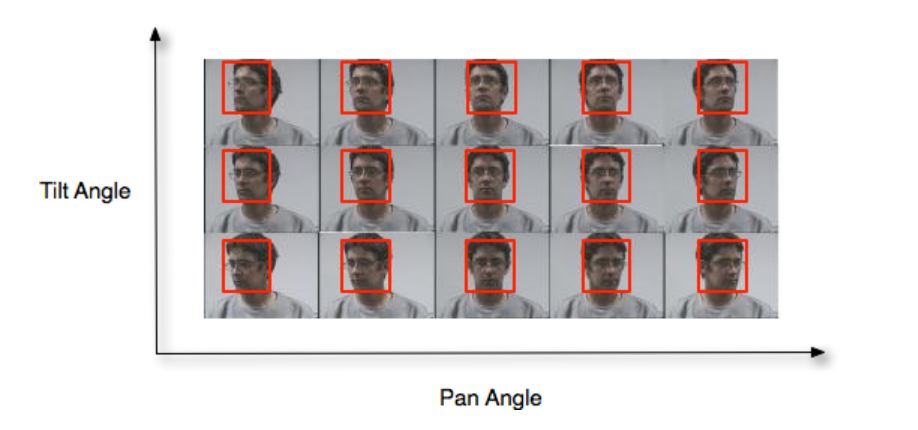
\includegraphics[scale=1]{figures/tiltpan.png}
	\caption{Muestra de 15 fotografías del sujeto 12 \cite{Gourier_Hall_Crowley}}
	\label{fig:img0}
\end{figure}

\begin{figure}[H]
	\centering
	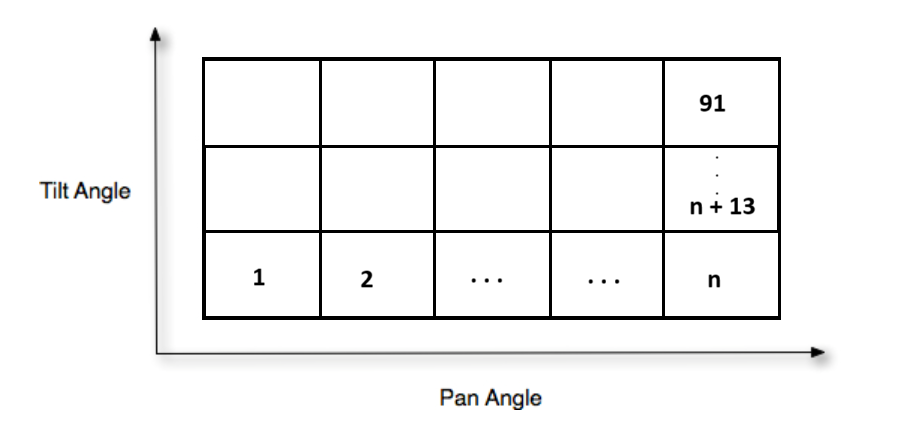
\includegraphics[scale=1]{figures/faceorder.png}
	\caption{Orden de guardado para cada serie de fotografías}
	\label{fig:img1}
\end{figure}

Además de este orden, todas las series de fotografías iniciaban con la imagen de la cabeza completamente hacia arriba y finalizaban con la posición completamente abajo, de frente para ambas. Dado que se tenían 15 sujetos de prueba, se procedió a guardar los archivos JPG de 11 (2046 imágenes) sujetos en un directorio de entrenamiento y los 4 (744 imágenes) restantes en el de pruebas. Al tener en cuenta el orden de los archivos y la cantidad en cada directorio se procedió a realizar las etiquetas por medio de un documento \textit[Excel]con formato \textit[.xlsx]. En dicho documento se creó una hoja para cada grupo de etiquetas, esto quiere decir, una hoja para etiquetas de entrenamiento y otra para etiquetas de prueba.

\subsubsection{Etiquetas para clasificación}

Para la primera experimentación se consideró clasificar las imágenes en 9 clases diferentes, de tal manera que la orientación de la cabeza respecto de la cámara funcionara de manera similar a una palanca de mandos analógica. A continuación se presenta una visualización de dicha clasificación:

\begin{figure}[H]
	\centering
	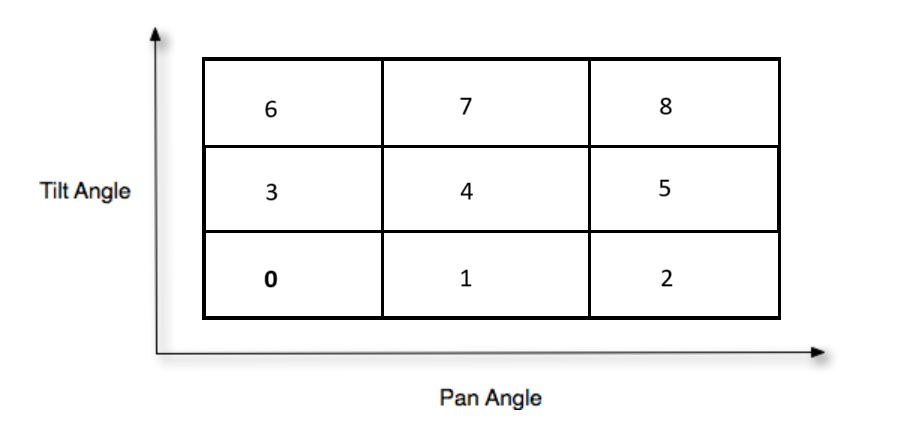
\includegraphics[scale=1]{figures/clasi0.png}
	\caption{Clasificación de imágenes en 9 etiquetas}
	\label{fig:img2}
\end{figure}

Utilizando esta cantidad de clases, se realizaron dos formas de etiquetado en las imágenes, en las cuales solo varía la cantidad de fotografías que fueron etiquetadas dentro de una clase u otra. En las siguientes figuras se podrá observar que la dimensión de cada celda está representada con (n $\times$ m), dónde n corresponde a la cantidad de ángulos panorámicos que abarca y m la cantidad de ángulos de inclinación (según las muestras tomadas del ICPR). Además, la posición de las celdas en las gráficas si corresponde a la numeración de la Figura 2.


\begin{figure}[H]
	\centering
	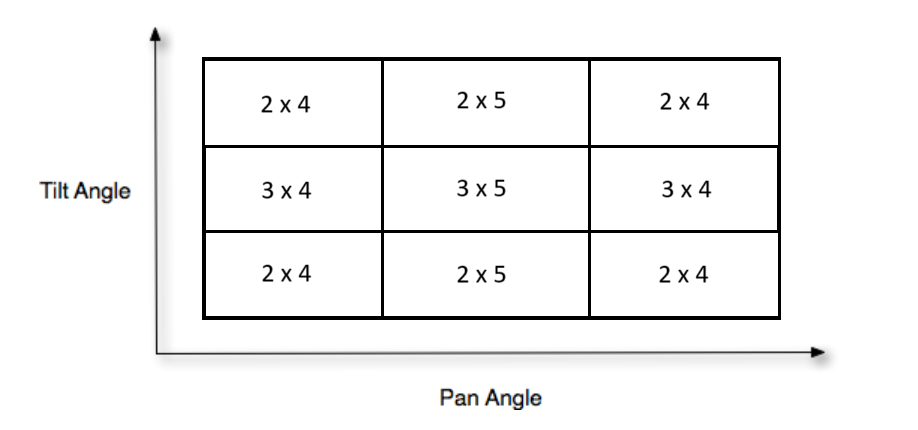
\includegraphics[scale=1]{figures/clasi01.png}
	\caption{Primera distribución de etiquetas}
	\label{fig:img3}
\end{figure}

\begin{figure}[H]
	\centering
	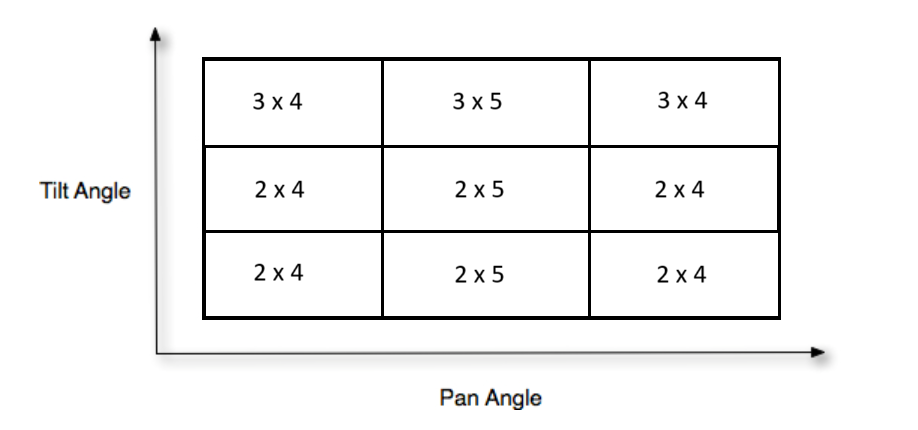
\includegraphics[scale=1]{figures/clasi02.png}
	\caption{Segunda distribución de etiquetas}
	\label{fig:img4}
\end{figure}

Luego de pruebas realizadas con resultados no satisfactorios en la sección de algoritmos para visión por computadora, la siguiente experimentación consistió en reducir la cantidad de clases a 6. En este caso los movimientos hacia atrás no funcionan como retroceso sino por medio de un giro completo del agente móvil. Y la clasificación resultante se muestra a continuación:

\begin{figure}[H]
	\centering
	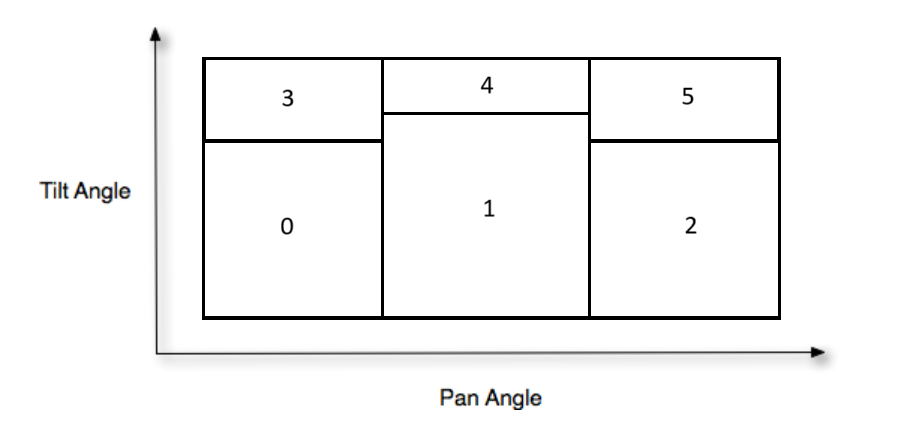
\includegraphics[scale=1]{figures/clasi1.png}
	\caption{Clasificación de imágenes en 6 etiquetas}
	\label{fig:img5}
\end{figure}

\begin{figure}[H]
	\centering
	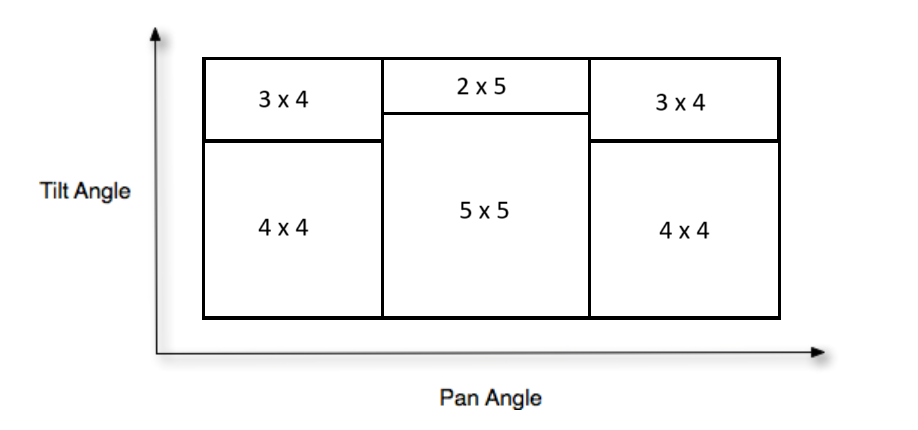
\includegraphics[scale=1]{figures/clasi2.png}
	\caption{Tercera distribución de etiquetas}
	\label{fig:img6}
\end{figure}

\begin{figure}[H]
	\centering
	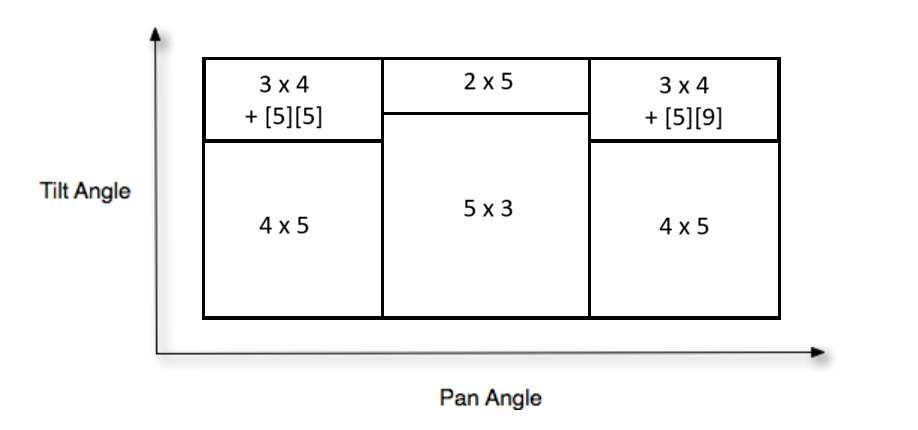
\includegraphics[scale=1]{figures/clasi3.png}
	\caption{Cuarta distribución de etiquetas (Las posiciones se cuentan desde la esquina inferior izquierda)}
	\label{fig:img7}
\end{figure}


\section{Algoritmos para visión por computadora}


\chapter{Algoritmo de traducción}

%Esta etapa contempla la iteración de pruebas para conseguir un algoritmo que funcione de manera efectiva al reconocer los gestos y movimientos de la cabeza del usuario. Luego de obtener un reconocimiento efectivo, se generarán diferentes ítems, clases o divisiones para cada tipo de gestos. Al tener definida la lista de tipos, se procede a utilizarlos para generar comandos genéricos para poder utilizar los agentes robóticos móviles simulados y físicos.

\chapter{Simulaciones}

%El algoritmo anterior será utilizado para realizar simulaciones de movimiento/envío de comandos en diferentes escenarios. Para poder ejecutar dichas pruebas, será necesario también realizar un análisis de los diferentes simuladores disponibles, los cuales sean compatibles con los algoritmos determinados anteriormente. Se realizará un registro de datos de las iteraciones realizadas para analizarlas de manera estadísticas y determinar el comportamiento de cada algoritmo según el escenario propuesto. De esta manera, se podrá partir con datos o comandos iniciales para las pruebas físicas. Los escenarios a probar constan del entorno físico alrededor del robot, así como los diferentes gestos a utilizar. 

\chapter{Pruebas físicas}

%Al obtener los parámetros iniciales determinados en las simulaciones, se empezará la migración de estos, junto con los algoritmos, hacia los robots a utilizar. En primer lugar se realizará una comparación entre los resultados obtenidos de manera física contra las simulaciones. Las pruebas físicas se realizarán en diferentes condiciones, como el de luminosidad, o el de contenido visual con diferentes niveles de ruido para tener un rango de operación más grande. También, las pruebas físicas tendrán un análisis cada algoritmo con diferentes variaciones en parámetros iniciales o en el algoritmo por sí mismo. De esta manera se podría verificar el alcance del sistema en conjunto, del robot, el sensor y el algoritmo seleccionado. También, se realizarán pruebas con diferentes sujetos de control, es decir diferentes personas realizando los gestos para controlar el movimiento del robot. Al realizar las pruebas, también se guardaran los datos obtenidos a partir de los sensores de tal manera que se puedan clasificar dependiendo del gesto utilizado. 
